\section{Microcontrôleur}

\subsection{Introduction}

\subsection{Microprocesseur (\textit{µP})}
Un \textbf{microprocesseur} (\textit{µP}) est une 
\textbf{unité centrale de traitement} (\textbf{CPU}\footnote{Glossaire : \gls{cpu}}) qui exécute des 
instructions, mais qui \textbf{ne contient ni mémoire RAM, ni mémoire ROM, ni 
entrées/sorties intégrées}. Il est conçu pour des systèmes où ces composants, 
tels que la \textit{RAM}, la \textit{ROM}, et les \textit{interfaces}, sont 
ajoutés séparément sur une carte mère. Le \textit{microprocesseur} est 
principalement utilisé dans les \textbf{ordinateurs}, \textbf{serveurs}, et 
\textbf{systèmes embarqués avancés}, comme les processeurs Intel, AMD, ou Apple 
Silicon.\par

\subsection{Microcontrôleur (\textit{MCU})}
Un \textbf{microcontrôleur} (\textit{MCU}) est un \textbf{circuit intégré complet} 
qui inclut non seulement un \textbf{microprocesseur}, mais aussi de la 
\textbf{mémoire RAM}, de la \textbf{mémoire ROM (Flash)} et des 
\textbf{périphériques d'entrées/sorties} sur une seule puce. Cela lui confère un 
\textbf{plus haut degré d'intégration} par rapport à un microprocesseur. Il est 
également appelé un \textbf{Système sur une Puce} (\textbf{SoC}, 
\textit{System On a Chip}). Il est conçu pour exécuter des 
\textbf{tâches spécifiques} à un \textbf{coût réduit} et avec une 
\textbf{consommation d'énergie optimisée}. On le retrouve dans des 
\textbf{systèmes embarqués}, notamment dans des 
\textbf{appareils électroménagers}, des \textbf{voitures}, des 
\textbf{jouets électroniques}, et des \textbf{objets connectés}, comme les 
dispositifs basés sur \textit{Arduino}, \textit{STM32}, \textit{PIC}, et 
\textit{ESP32}.\par

\section{Le microcontrôleur ESP32}

Le microcontrôleur utilisé dans la mineure \textbf{Instrumentation} est 
l'\textbf{ESP32}, fabriqué par \textbf{Espressif Systems} (\textit{Chine}).

\subsection{Caractéristiques principales de l'ESP32}
Le \textbf{processeur} de l'ESP32 est un \textit{Dual-Core Xtensa LX6} qui peut 
fonctionner jusqu'à \SI{240}{\mega\hertz}, conçu par \textbf{Tensilica}. Il
dispose également d' \textbf{instructions DSP} (\textit{Digital Signal Processing}) 
intégrées, permettant le \textbf{traitement de signaux complexes}. En termes de 
\textbf{connectivité}, l'ESP32 supporte le \textbf{Wi-Fi}, le \textbf{Bluetooth}, 
ainsi que le \textbf{Bluetooth Low Energy (BLE)}. Il dispose également de 
\textbf{modes basse consommation}, ce qui est crucial pour les applications à 
faible consommation énergétique. Parmi les \textbf{interfaces de périphériques} 
disponibles, on trouve :
\begin{itemize}
    \item \textbf{CAN} (Convertisseur \textbf{DAC})
    \item \textbf{CNA} (Convertisseur \textbf{ADC})
    \item \textbf{Capteur de toucher}
    \item \textbf{SPI}, \textbf{I2C}, \textbf{I2S}, \textbf{CAN}, \textbf{UART}, \textbf{PWM}
\end{itemize}

\begin{figure}[!ht]
    \centering
    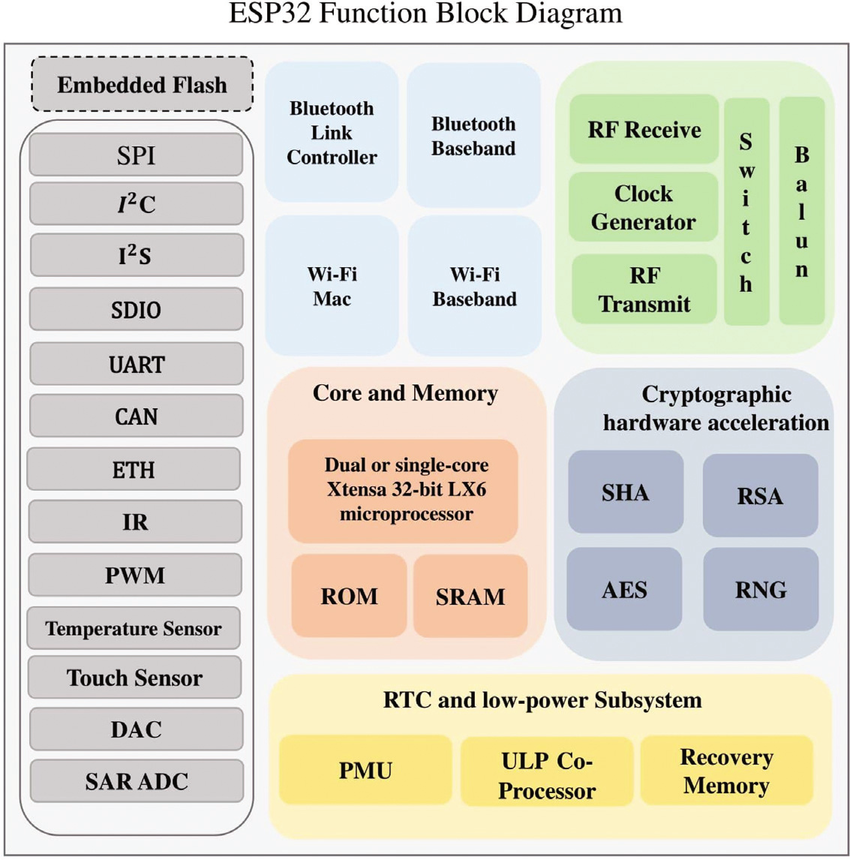
\includegraphics[width=0.9\textwidth]{esp32-block}
    \caption{Microcontrôleur ESP32}
    \label{fig:esp32}
\end{figure}

\subsection{Carte de développement ESP32-WROVER-B}
Le \textbf{microcontrôleur ESP32} est intégré dans une
 \textbf{carte de développement} basée sur le module \textbf{ESP32-WROVER-B}, 
 fabriqué par \textbf{uPesy} (\textit{France}), sous la référence 
 \textbf{ESP32 Wrover DevKit v2.1}. Cette carte présente plusieurs 
 \textbf{avantages} :
\begin{itemize}
    \item \textbf{Brochage des principales entrées/sorties}, facilitant ainsi son utilisation pour le prototypage.
    \item \textbf{Alimentation et connexion USB-C} intégrées pour un usage simplifié.
    \item \textbf{Mémoire supplémentaire} pour des applications plus complexes.
    \item \textbf{Compatibilité breadboard}, idéale pour la réalisation de \textbf{prototypes}.
\end{itemize}